%%% Copyright (C) 2018 Vincent Goulet
%%%
%%% Ce fichier fait partie du projet
%%% «Rédaction avec LaTeX»
%%% http://github.com/vigou3/formation-latex-ul
%%%
%%% Cette création est mise à disposition selon le contrat
%%% Attribution-Partage dans les mêmes conditions 4.0
%%% International de Creative Commons.
%%% http://creativecommons.org/licenses/by-sa/4.0/

\chapter{Bibliographie et citations}
\label{chap:bibliographie}

\nobibliography*

La production de la bibliographie d'un ouvrage d'une certaine ampleur
--- qu'il s'agisse d'un article scientifique, d'un mémoire, d'une
thèse --- est une tâche d'une grande importance qui peut rapidement devenir
laborieuse\dots\ lorsqu'elle n'est pas réalisée avec les outils appropriés.

L'ordinateur est bien meilleur qu'un humain pour accomplir certaines
opérations propres à la production d'une bibliographie. Un auteur ne
devrait se préoccuper que de colliger les informations
bibliographiques, puis de sélectionner les ouvrages à citer. La
machine peut ensuite se charger:
\begin{itemize}
\item d'inclure dans la bibliographie tous les ouvrages cités dans le
  document et seulement ceux-ci;
\item de trier les entrées de la bibliographie;
\item de composer les entrées de manière uniforme;
\item de recommencer ces opérations autant de fois que nécessaire pour
  un même document ou pour chaque nouveau document.
\end{itemize}

Avec en main une base de données bibliographique, la création de la
bibliographie devient une tâche triviale qui ne prend guère plus que
les quelques secondes de compilation nécessaires pour la composer.



\section{Quel système utiliser?}
\label{sec:bibliographie:systeme}

La gestion des citations et la composition d'une bibliographie sont
des tâches hautement spécialisées. Comme la plupart des traitements de
texte, {\LaTeX} les confie donc à des outils externes. Reste à savoir
lequel de ces outils utiliser.

%% hack ici pour afficher le logo BibTeX en police sans serif qui n'a
%% pas de version petites capitales tout en utilisant la commande
%% usuelle dans la table des matières
\subsection[{\BibTeX} et \pkg{natbib}]{%
  {B\kern-.025em{\small I}\kern-.025em{\small  B}\kern-.08em\TeX} %
  et \pkg{natbib}}
\label{sec:bibliographie:systeme:bibtex}

Fort de plus de 25 années d'existence, {\BibTeX}\index{bibtex@\BibTeX}
\citep{bibtex} est le système standard de traitement des
bibliographies dans {\LaTeX}. Il est stable et prévisible --- ce que
certains considéreraient des bogues passent pour des caractéristiques
--- et, surtout, il existe un vaste catalogue de références
bibliographiques en format {\BibTeX}. C'est généralement le seul
format accepté par les revues scientifiques. Non qu'il s'agisse d'un
argument massue, mais même Wikipedia, dans les rubriques «Citer cette
page», et la Bibliothèque de l'Université Laval, dans les pages de
notices bibliographiques, offrent les citations en format {\BibTeX}.

{\BibTeX} est principalement un système de tri d'entrées
bibliographiques et d'interface avec la base de données. La
présentation des citations et de la bibliographie relève d'un
\emph{style}. Les styles standards sont \code{plain}, \code{unsrt},
\code{alpha} et \code{abbrv}; nous y reviendrons à la
\autoref{sec:bibliographie:style}.

Fonctionnant de pair --- et exclusivement --- avec {\BibTeX},
\pkg{natbib} \citep{natbib} est un paquetage qui fournit des styles et
des commandes pour composer des bibliographies dans le format
auteur-année fréquemment utilisé dans les sciences naturelles et
sociales\footnote{%
  C'est le style utilisé dans le présent document.}. %
Le paquetage est également compatible avec les styles de citation
standards mentionnés ci-dessus.

Parce qu'il est flexible et qu'il rend facile de produire des
extensions compatibles, \pkg{natbib} est en quelque sorte devenu un
standard \emph{de facto} pour la composition des bibliographies.
D'ailleurs, la classe \class{ulthese} pour les thèses et mémoires de
l'Université Laval charge par défaut le paquetage.

Il existe plusieurs autres paquetages pour rencontrer des exigences
particulières avec {\BibTeX}: bibliographies multiples, bibliographies
par chapitre, etc. \citet{Mori:bibliographies:2009} en offre un bon
survol. Consulter aussi la section \emph{Bibliographies and citations}
de la formidable %
\doc[\emph{UK List of {\TeX} Frequently Asked Questions}]{letterfaq}{http://www.tex.ac.uk/}.


\subsection{Biber et biblatex}
\label{sec:bibliographie:systeme:biblatex}

Au moment d'écrire ces lignes, un nouveau système de traitement des
bibliographies dans {\LaTeX} est en émergence. Il est formé du moteur
de traitement Biber\index{Biber} \citep{biber} et du paquetage \pkg{biblatex}\index{biblatex}
\citep{biblatex}. Ensemble, ils visent tout à la fois à remplacer
l'infrastructure bâtie autour de {\BibTeX} et à proposer des
fonctionnalités additionnelles. Citons le support natif des caractères
UTF-8 et de nombreux modes de citation, dont le mode
auteur-titre populaire en sciences humaines.

Le duo Biber-\pkg{biblatex} bénéficie d'un développement récent en
phase avec les technologies et les préoccupations actuelles. Certains
enjoignent aux débutants de sauter dans ce train. Difficile,
cependant, de dire si ce système saura s'établir comme nouveau
standard, surtout compte tenu de la masse de matériel disponible pour
{\BibTeX}.

Pour de l'information additionnelle, consulter %
\link{http://tex.stackexchange.com/questions/25701/bibtex-vs-biber-and-biblatex-vs-natbib}{cette entrée} %
du site {\TeX}--{\LaTeX} Stack Exchange qui fournit un excellent
sommaire des mérites et des inconvénients respectifs des deux systèmes
de traitement de bibliographie.

En l'absence d'un consensus clair, nous avons choisi de traiter dans
ce chapitre à la fois du système le plus répandu et de celui avec
lequel nous sommes le plus familier, soit la combinaison {\BibTeX} et
\pkg{natbib}.

\subsection{EndNote}
\label{sec:bibliographie:systeme:endnote}

EndNote\index{EndNote} est un logiciel commercial de gestion bibliographique très
répandu dans certaines disciplines scientifiques. Il n'est donc pas
rare que les nouveaux utilisateurs de {\LaTeX} demandent: «puis-je
utiliser EndNote pour ma bibliographie?» La réponse courte est «Non»,
car {\LaTeX} ne peut traiter directement les données bibliographiques
de EndNote. La réponse plus longue est «Oui, indirectement»,
car EndNote possède un filtre pour exporter ses données en format
{\BibTeX}.

Il est hors de la portée de ce document de traiter de la conversion
des données bibliographiques de EndNote. Une simple recherche dans
Internet sur «EndNote BibTeX» devrait fournir toute l'information
nécessaire pour réaliser la conversion.


\section{Processus de création d'une bibliographie}
\label{sec:bibliographie:processus}

La création d'une bibliographie compte plusieurs étapes. Nous les
présentons ici afin d'en avoir une vue d'ensemble avant d'aborder les
détails dans les sections suivantes.

\begin{enumerate}
\item Construire une ou plusieurs bases de données contenant les
  informations bibliographiques. On utilise les mêmes bases de données
  pour tous ses documents. Par conséquent, le temps consacré à cette
  étape s'amenuise au fur et à mesure que l'on complète ses bases de
  données.
\item Choisir un style de citation et de présentation de la
  bibliographie, généralement en se conformant aux us et coutumes dans
  sa discipline scientifique ou aux instructions d'un éditeur.
\item Insérer dans le texte de son document des références à des
  ouvrages se trouvant dans ses bases de données bibliographiques.
\item Insérer dans le code source du document les informations
  relatives au style de bibliographie et aux bases de données à
  utiliser, puis composer les références et la bibliographie avec
  {\BibTeX}.
\end{enumerate}


\section{Création d'une base de données}
\label{sec:bibliographie:bib}

Il est tout à fait possible de citer des références et de construire
une bibliographie avec {\LaTeX} sans avoir recours à une base de
données bibliographiques et à {\BibTeX} pour traiter celles-ci. Nous
recommandons toutefois fortement d'adopter cette approche.
L'investissement requis en temps et en efforts demeure relativement
faible, surtout au regard des avantages:
\begin{itemize}
\item on entre les informations dans une base de données une seule
  fois pour ensuite les utiliser à répétition;
\item le traitement automatisé des informations assure une
  présentation uniforme de celles-ci;
\item on peut changer le style de présentation de la bibliographie
  sans pour autant toucher aux informations bibliographiques.
\end{itemize}

La base de données n'est en fait qu'un simple fichier texte dans
lequel sont regroupées dans un format précis les informations
bibliographiques. Le nom du fichier doit nécessairement comporter
l'extension \code{.bib}.

La base de données est composée d'entrées de divers \emph{types}:
livre, article scientifique, thèse, etc. Chaque entrée comporte un
certain nombre de \emph{champs}: titre, nom de l'auteur, date de
publication, etc. Pour un type d'entrée donné, certains champs sont
obligatoires, d'autres optionnels et d'autres simplement ignorés ou
inactifs.

La structure générale d'une entrée de base de données est la suivante:
\begin{lstlisting}
@`\meta{type\_entree}'{`\meta{clé}',
  `\marg{champ}' = `\marg{valeur}',
  ...,
  `\marg{champ}' = `\marg{valeur}'}
\end{lstlisting}
Ci-dessus, \meta{clé} est un identifiant arbitraire, mais unique ---
et idéalement mnémonique --- de l'entrée. C'est cette clé qui sera
utilisée pour faire référence à l'entrée dans le code source du
document.

Il est beaucoup plus facile de comprendre ce dont il est question ici
par le biais d'exemples. Des commentaires et précisions additionnels sur la
préparation des entrées bibliographiques suivent l'\autoref*{ex:bibliographie:bib}.

\begin{exemple}
  \label{ex:bibliographie:bib}
  On trouvera ci-dessous les entrées bibliographiques d'un livre
  \citep{Kopka:latex:4e}, d'un article scientifique
  \citep{Mori:bibliographies:2009} et d'un manuel générique, en
  l'occurrence la documentation d'un paquetage \citep{natbib}. Pour
  faciliter la comparaison, chaque entrée est immédiatement suivie du
  texte de la notice tel qu'il apparaît dans la bibliographie du
  présent ouvrage.

\begin{lstlisting}[language=]
@Book{Kopka:latex:4e,
  author =    {Kopka, Helmut and Daly, Patrick W.},
  title =     {Guide to {\LaTeX}},
  publisher = {Addison-Wesley},
  year =      2003,
  edition =   4,
  isbn =      {978-032117385-0},
  language =  {english}}
\end{lstlisting}

  \begin{framed}
    \noindent \nolink{\bibentry{Kopka:latex:4e}}.
  \end{framed}

\begin{lstlisting}[language=]
@Article{Mori:bibliographies:2009,
  author =   {Lapo F. Mori},
  title =    {Managing bibliographies with {\LaTeX}},
  journal =  {{TUG}boat},
  year =     2009,
  volume =   30,
  number =   1,
  pages =    {36-48},
  url =	{https://www.tug.org/TUGboat/tb30-1/tb94mori.pdf},
  language = {english}}
\end{lstlisting}

  \begin{framed}
    \noindent \nolink{\bibentry{Mori:bibliographies:2009}}.
  \end{framed}

\begin{lstlisting}[language=]
@Manual{natbib,
  author =   {Patrick W. Daly},
  title =    {Natural Sciences Citations and References},
  year =     2010,
  url =      {http://www.ctan.org/pkg/natbib/},
  language = {english}}
\end{lstlisting}

  \begin{framed}
    \noindent \nolink{\bibentry{natbib}}.
  \end{framed}
  \qed
\end{exemple}


\begin{itemize}
\item Les types d'entrée bibliographique dans l'exemple ci-dessus sont
  \code{Book}, \code{Article} et \code{Manual}\footnote{%
    Les identifiants des types d'entrée et des champs sont insensibles
    à la casse. Par exemple, on pourrait tout aussi bien débuter une
    entrée par \code{@Manual}, \code{@manual} ou \code{@MANUAL}.}. %
  On remarquera que les champs utilisés sont différents d'un type à un
  autre.

  On trouvera la liste de tous les types d'entrée et des champs
  obligatoires et optionnels pour chacun dans, entre autres, %
  \doc[Wikipedia]{}{https://fr.wikipedia.org/wiki/BibTeX}, %
  la %
  \doc[documentation de {\BibTeX}]{btxdoc}{http://www.texdoc.net/pkg/btxdoc} %
  ou la plupart des bons ouvrages de référence
  \citep[comme][]{Kopka:latex:4e}.
\item On entre le nom d'un auteur soit sous la forme \code{\{Prénom
    Nom\}}, soit sous la forme \code{\{Nom, Prénom\}}. La seconde
  forme est surtout utile pour distinguer explicitement le nom du
  prénom, par exemple dans le cas de prénoms ou de noms multiples.
\item Lorsqu'un ouvrage compte plusieurs auteurs, on distingue ceux-ci
  en séparant le nom complet de \emph{chacun} des auteurs par le
  mot-clé \code{and}.
\item {\BibTeX} gère automatiquement les hauts et bas de
  casse (majuscules et minuscules), en particulier dans les titres
  d'ouvrages. Pour préserver une casse particulière, il suffit de
  placer les lettres entre accolades.

  Par exemple, dans la seconde entrée de
  l'\autoref{ex:bibliographie:bib}, le titre du journal TUGboat est
  inscrit sous la forme \code{\{\{TUG\}boat\}} pour éviter que {\BibTeX}
  ne le transforme en «Tugboat».
\item Les champs \code{isbn}, \code{url} et quelques autres
  \citep[section~2.8]{natbib} sont fournis par le paquetage
  \pkg{natbib}. Même si ces champs ne devaient pas s'afficher dans la
  bibliographie pour le style choisi, c'est une bonne idée d'insérer
  les informations dans la base de données pour référence future.
\item Le champ \code{language}, introduit par \pkg{babel}, permet de
  préciser la langue de l'entrée bibliographique. La césure de mots et
  la composition de certains éléments seront ainsi adaptées en
  conséquence.

  Par exemple, si l'entrée d'un document comporte le champ
  \code{edition = 2}, sa fiche bibliographique contiendra la mention
  «2{\ieme} édition» ou «2\up{nd} edition» selon que l'on a précisé
  que l'ouvrage est en français ou en anglais.
\item {\BibTeX} supporte les lettres accentuées ou autres caractères
  spéciaux dans le texte des champs seulement si le document utilisant
  la bibliographie supporte lui-même ces caractères; voir la
  \autoref{sec:bases:francais}. Autrement, il faut entrer les
  caractères spéciaux avec les commandes {\LaTeX} de base tel
  qu'expliqué sommairement à la \autoref{sec:bases:caracteres}.

  Notre recommandation: éviter les lettres accentuées dans les
  entrées susceptibles d'être utilisées dans un document entièrement
  en anglais.
\end{itemize}

\tipbox{Entretenir une base de données bibliographiques unique peut
  rapidement devenir pénible quand le nombre d'entrée devient grand.

  Mieux vaut alors scinder ses références dans plusieurs fichiers par
  thématique, un peu comme dans une bibliothèque:
  droit, finance, informatique, mathématiques, etc.

  On nommera ensuite les fichiers du nom de la thématique:
  \code{droit.bib}, \code{finance.bib},
  \code{informatique.bib}, etc.}



\section{Style des citations et de la bibliographie}
\label{sec:bibliographie:style}

Il existe plusieurs manières différentes de présenter une
bibliographie et {\LaTeX} sait s'adapter. Le format général de la
bibliographie est contrôlé par un \emph{style} choisi avec la commande
\cmd{\bibliographystyle}. Le style affecte habituellement deux
composantes de la bibliographie:
\begin{enumerate}
\item le mode de citation dans le texte (numérique, alphanumérique,
  auteur-année, etc.);
\item la présentation des notices bibliographiques (ordre des
  éléments, ponctuation, mise en forme des caractères, etc.).
\end{enumerate}
On trouvera des exemples de quelques styles de bibliographie dans le
\autoref{tab:bibliographie:styles}.

\begin{table}
  \caption{Quelques styles de bibliographie et leur effet sur le mode de
    citation et le format des notices bibliographiques}
  \label{tab:bibliographie:styles}
  \small
  \textbf{Styles standards numériques et alphanumériques} \\[0.5\normalbaselineskip]
  \begin{tabularx}{1.0\linewidth}{p{0.16\linewidth}p{0.35\linewidth}X}
    \toprule
    style & mode de citation & format de notice \\
    \midrule
    \code{plain} &
    Un bon ouvrage de référence est [1]  &
    \begin{bibexample}
    \item[{[1]}] Helmut Kopka and Patrick~W. Daly.
      \emph{Guide to {\LaTeX}}. Addison-Wesley, 4 edition, 2003.
    \end{bibexample}
    \\ \addlinespace[8pt]
    \code{plain-fr} &
    Un bon ouvrage de référence est [1] &
    \begin{bibexample}
    \item[{[1]}] Helmut \textsc{Kopka} et Patrick~W. \textsc{Daly}:
      \emph{Guide to {\LaTeX}}. Addison-Wesley, 4 édition, 2003.
    \end{bibexample}
    \\ \addlinespace[8pt]
    \code{alpha-fr} &
    Un bon ouvrage de référence est [KD03] &
    \begin{bibexample}
    \item[{[KD03]}] Helmut \textsc{Kopka} et Patrick~W. \textsc{Daly}:
      \emph{Guide to {\LaTeX}}. Addison-Wesley, 4 édition, 2003.
    \end{bibexample} \\
  \end{tabularx} \\
  \medskip

  \textbf{Styles auteur-année avec \pkg{natbib}} \\[0.5\normalbaselineskip]
  \begin{tabularx}{1.0\linewidth}{p{0.16\linewidth}p{0.35\linewidth}X}
    \toprule
    style & mode de citation & format de notice \\
    \midrule
    \code{plainnat-fr} &
    Un bon ouvrage de référence est Kopka et Daly (2003)  &
    \begin{bibexample}
    \item[] Helmut \textsc{Kopka} et Patrick~W. \textsc{Daly}:
      \emph{Guide to {\LaTeX}}. Addison-Wesley, 4 édition, 2003.
    \end{bibexample}
    \\ \addlinespace[8pt]
    \code{francais} &
    Un bon ouvrage de référence est Kopka et Daly (2003)  &
    \begin{bibexample}
    \item[] Kopka, H.\ et P.~W. Daly. 2003.
      \emph{Guide to {\LaTeX}}, 4{\ieme} éd., Addison-Wesley.
    \end{bibexample} \\
    \bottomrule
  \end{tabularx}
\end{table}

Les styles standards de {\LaTeX} sont \code{plain}, \code{unsrt},
\code{alpha} et \code{abbrv}. Ces styles ont été développés pour des
modes de citation numériques ou alphanumériques.

Pour plus de flexibilité, nous recommandons d'utiliser le paquetage
\pkg{natbib} pour la gestion des références et du style de la
bibliographie. Entre autres choses, ce paquetage supporte le style de
citation auteur-année fréquemment employé en sciences naturelles et
sociales, plusieurs commandes de citation, un grand nombre de styles
de bibliographie, ainsi que des entrées spécifiques pour les numéros
ISBN et les URL. Le paquetage fournit des styles \code{plainnat},
\code{unsrtnat} et \code{abbrvnat} similaires aux styles standards,
mais plus complets. Il existe des %
\doc[versions francisées]{}{http://mirrors.ctan.org/biblio/bibtex/contrib/bib-fr/} %
de ces styles dans CTAN et dans {\TeX}~Live.
Il est fortement recommandé de consulter la %
\doc{natbib}{http://texdoc.net/pkg/natbib/} %
de \pkg{natbib} pour les détails. On y trouvera également des
informations sur l'utilisation de styles de citation autres que
auteur-année.

Également dans CTAN et dans {\TeX}~Live, le paquetage
\pkg{francais-bst} \citep{francais-bst} fournit deux feuilles de style
compatibles avec \pkg{natbib} permettant de composer des
bibliographies auteur-année respectant les normes de typographie
française proposées dans \citet{Malo:1996}; voir le dernier exemple du
\autoref{tab:bibliographie:styles}.

Le paquetage \pkg{natbib} est chargé par défaut par la classe
\class{ulthese}; consulter la section~6.6 de la %
\doc{ulthese}{http://texdoc.net/pkg/ulthese/} %
de la classe pour plus d'information sur l'interaction entre le
paquetage et celle-ci.

En terminant, notons que la plupart des journaux scientifiques et des
maisons d'édition ont leur propre style que les auteurs sont tenus
d'utiliser. En ce qui a trait aux thèses et mémoires de l'Université
Laval, la Faculté des études supérieures et postdoctorales n'impose
aucun style de bibliographie particulier. Nous recommandons
d'utiliser le style usuel dans sa discipline scientifique.



\section{Insertion de références dans le texte}
\label{sec:bibliographie:cite}

La raison première d'une bibliographie, c'est évidemment d'y colliger
les informations relatives aux ouvrages auxquels un document fait
référence. Avant de penser créer une bibliographie, il faut donc
savoir comment insérer des références dans le texte.

La commande de base pour insérer une référence au fil du texte dans
{\LaTeX} est
\begin{lstlisting}
\cite`\marg{clé}'
\end{lstlisting}
L'effet de la commande est double:
\begin{enumerate}
\item insérer une référence comme «\nolink{\citet{Mori:bibliographies:2009}}»
  dans le texte;
\item ajouter le document dans la bibliographie.
\end{enumerate}
En somme, outre la phase de compilation qui fait l'objet de la section
suivante, c'est tout ce qu'il y a à faire pour construire sa
bibliographie.

Avec \pkg{natbib}, on utilisera plutôt les commandes
\begin{lstlisting}
\citet`\marg{clé}'
\citep`\marg{clé}'
\end{lstlisting}
Dans le style de citation auteur-année, ces commandes permettent
respectivement d'insérer une référence au fil de la phrase ou en
aparté:
\begin{demo}
  \begin{texample}[0.55\linewidth]
\begin{lstlisting}
\citet{Mori:bibliographies:2009}
en offre un bon survol.
\end{lstlisting}
    \producing
    \citet{Mori:bibliographies:2009},
    en offre un bon survol.
  \end{texample}
  \begin{texample}[0.55\linewidth]
\begin{lstlisting}
TUGboat a publié un bon survol
\citep{Mori:bibliographies:2009}.
\end{lstlisting}
    \producing
    TUGboat a publié un bon survol
    \citep{Mori:bibliographies:2009}.
  \end{texample}
\end{demo}

On ne devrait \emph{jamais} entrer directement dans le texte des
informations bibliographiques, même partielles. Pour insérer dans le
texte le nom d'un auteur ou l'année de publication d'un ouvrage,
\pkg{natbib} offre les commandes:
\begin{lstlisting}
\citeauthor`\marg{clé}'
\citeyear`\marg{clé}'
\end{lstlisting}
Avec ces commandes, pas de risque de mal orthographier un nom par
inadvertance, ou d'oublier de modifier dans le texte une année de
publication que l'on aura changé dans la base de données
bibliographique.

Le paquetage fournit plusieurs autres commandes pour manipuler les
informations bibliographiques et contrôler leur présentation;
consulter la %
\doc{natbib}{http://www.texdoc.net/pkg/natbib} %
de \pkg{natbib}.

Il arrive que l'on souhaite inclure dans la bibliographie un ou
plusieurs documents qui ne sont pas cités dans le texte. Pour ce
faire, insérer dans le corps du document la commande
\begin{lstlisting}
\nocite`\marg{clé1,clé2,...}'
\end{lstlisting}
où \meta{clé1}, \meta{clé2}, \dots, sont les clés des documents à
inclure dans la bibliographie.

\begin{figure}[t]
  \begin{emphbox}{Suppression des hyperliens indésirables}
    Le paquetage \pkg{hyperref} fait automatiquement d'une référence
    bibliographique un hyperlien vers l'entrée dans la bibliographie.
    C'est le cas dans le présent document.

    Il peut arriver que l'hyperlien soit superflu ou indésirable. Pour
    le supprimer pour une référence particulière, on utilise
    l'environnement \Ie{NoHyper}:
\begin{lstlisting}
\begin{NoHyper} \citet`\marg{clé}' \end{NoHyper}
\end{lstlisting}
    Pour usage fréquent, définir une nouvelle commande
    (\autoref{chap:commandes}). Par exemple, avec dans le préambule
\begin{lstlisting}
\newcommand{\nolink}[1]{%
  \begin{NoHyper}#1\end{NoHyper}}
\end{lstlisting}
    on pourra utiliser dans le texte
\begin{lstlisting}
\nolink{\citet`\marg{clé}'}
\end{lstlisting}
    pour supprimer l'hyperlien d'une référence bibliographique.
  \end{emphbox}
\end{figure}


\section{Composition de la bibliographie}
\label{sec:bibliographie:bibtex}

Les commandes de la section précédente servent à indiquer à {\LaTeX}
les ouvrages à inclure dans la bibliographie. C'est toutefois l'outil
externe {\BibTeX} qui se chargera de fournir à {\LaTeX} le texte des
références ainsi que le contenu de la bibliographie.

À la \autoref{sec:presentation:processus}, nous avons représenté
schématiquement comme suit le processus de création d'un document avec
pdf{\LaTeX} ou {\XeLaTeX}:
\begin{center}
  \sffamily
  \begin{minipage}[t]{0.12\linewidth}
    \centering
    {\LARGE\faFileTextO} \\ \medskip
    code source
  \end{minipage}
  \quad\faArrowRight\quad
  \begin{minipage}[t]{0.12\linewidth}
    \centering
    {\LARGE\faCogs} \\ \medskip
    \code{pdflatex} \\ \code{xelatex}
  \end{minipage}
  \quad\faArrowRight\quad
  \begin{minipage}[t]{0.12\linewidth}
    \centering
    {\LARGE\faFilePdfO} \\ \medskip
    fichier PDF
  \end{minipage}
\end{center}

Pour créer ou mettre à jour la bibliographie, il s'ajoute au processus
une étape de compilation du document avec {\BibTeX}:
\begin{center}
  \sffamily
  \begin{minipage}[t]{0.12\linewidth}
    \centering
    {\LARGE\faFileTextO} \\ \medskip
    code source
  \end{minipage}
  \quad\faArrowRight\quad
  \begin{minipage}[t]{0.12\linewidth}
    \centering
    {\LARGE\faCogs} \\ \medskip
    \code{pdflatex} \\ \code{xelatex}
  \end{minipage}
  \quad\faArrowRight\quad
  \begin{minipage}[t]{0.12\linewidth}
    \centering
    {\LARGE\faCogs} \\ \medskip
    \code{bibtex}
  \end{minipage}
  \quad\faArrowRight\quad
  \begin{minipage}[t]{0.12\linewidth}
    \centering
    {\LARGE\faCogs}\;
    \raisebox{-2pt}{\parbox[b]{1em}{\centering\large\faRepeat\tiny\\ $\times 2$}} \\ \medskip
    \code{pdflatex} \\ \code{xelatex}
  \end{minipage}
  \quad\faArrowRight\quad
  \begin{minipage}[t]{0.12\linewidth}
    \centering
    {\LARGE\faFilePdfO} \\ \medskip
    fichier PDF
  \end{minipage}
\end{center}

Plus en détails, le processus de préparation d'un document comprenant
une bibliographie est le suivant.

\begin{enumerate}
\item Composer le texte et y insérer des références avec les commandes
  de la section précédente.
\item Ajouter dans le préambule ou près de la commande
  \cmdprint{\bibliography} ci-dessous la commande
\begin{lstlisting}
\bibliographystyle`\marg{style}'
\end{lstlisting}
  où \meta{style} est un nom de style bibliographique.
\item Ajouter dans le texte la commande
\begin{lstlisting}
\bibliography{`\meta{base\_donnees1}', `\meta{base\_donnees2}', ...}
\end{lstlisting}
  à l'endroit où l'on veut qu'apparaisse la bibliographie
  (généralement à la fin du document). Les arguments
  \meta{base\_donnees1}, \meta{base\_donnees2}, séparés par des
  virgules, sont les noms (sans l'extension \code{.bib}) des fichiers
  de données bibliographiques.
\item \label{item:bibliographie:1} Compiler le document une première
  fois avec un moteur {\TeX} afin que {\LaTeX} détecte les ouvrages à
  insérer dans la bibliographie. À cette étape, les références dans le
  texte apparaissent sous forme d'un point d'interrogation
  «\textbf{?}».
\item Compiler le document avec {\BibTeX} afin de préparer le texte
  des références et composer la bibliographie.
\item \label{item:bibliographie:2} Compiler à nouveau le document au
  moins deux fois avec un moteur {\TeX} afin d'y insérer d'abord la
  bibliographie, puis le texte des références.
\end{enumerate}

Il faut répéter les étapes
\ref*{item:bibliographie:1}--\ref*{item:bibliographie:2} chaque fois
qu'une nouvelle référence est ajoutée dans le document ou que l'entrée
bibliographique est modifiée. Autrement, tant que la bibliographie
demeure inchangée, une compilation standard avec seulement le moteur
{\TeX} suffit.

\begin{exemple}
  La \autoref{fig:bibliographie:bibtex:1} présente le contenu d'un
  fichier de base de données bibliographiques et le fichier source
  d'un document simple contenant des références et une bibliographie.

  \begin{itemize}
  \item Le document utilise le mode de citation auteur-année de
    \pkg{natbib}.
  \item La présence du paquetage \pkg{fontspec} dans le préambule
    indique que le document doit être compilé avec {\XeLaTeX}. Cela
    fait en sorte que les lettres accentuées sont automatiquement
    supportées tant dans le texte que dans les entrées de la
    bibliographie.
  \item Le paquetage \pkg{babel} est activé avec l'anglais et le
    français, les deux langues utilisées dans la bibliographie. Nommé
    en dernier dans les options de chargement de la classe, le
    français est la langue par défaut du document.
  \end{itemize}

  Ces fichiers en main, les étapes de composition 1--3 sont
  complétées. La \autoref{fig:bibliographie:bibtex:2} présente la zone
  de texte principale du document après l'étape 4, puis après chacune
  des deux compilations de l'étape 6. %
  \qed
  \begin{figure}
    \centering
    \code{exemple-bibliographie.bib}
    \lstinputlisting[language=]{exemple-bibliographie.bib}
    \medskip
    \code{exemple-bibliographie.tex}
    \lstinputlisting[firstline=3]{exemple-bibliographie.tex}
    \caption{Code source d'un fichier de base de données (haut) et
      d'un document simple (bas)}
    \label{fig:bibliographie:bibtex:1}
  \end{figure}
  \begin{figure}
    \code{xelatex}
    \begin{framed}
      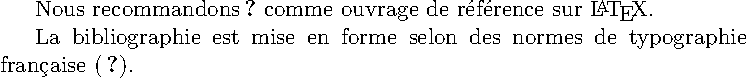
\includegraphics[width=\linewidth]{exemple-bibliographie-cropped-1}
    \end{framed}
    \code{xelatex} $\rightarrow$ \code{bibtex} $\rightarrow$ \code{xelatex}
    \begin{framed}
      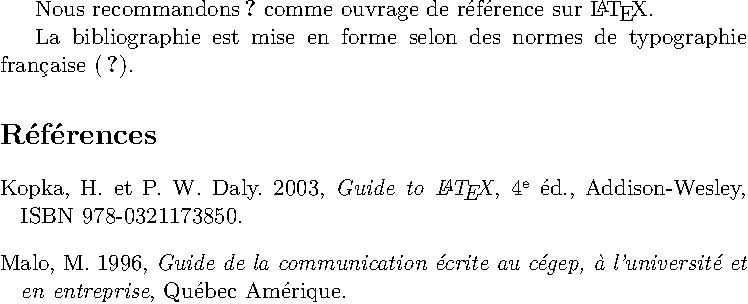
\includegraphics[width=\linewidth]{exemple-bibliographie-cropped-2}
    \end{framed}
    \code{xelatex} $\rightarrow$ \code{bibtex} $\rightarrow$ \code{xelatex} $\rightarrow$ \code{xelatex}
    \begin{framed}
      
\includegraphics[width=\linewidth]{exemple-bibliographie-cropped-3}
    \end{framed}
    \caption{Zone de texte du document aux diverses étapes de la
      compilation des fichiers de la
      \autoref{fig:bibliographie:bibtex:1} avec {\XeLaTeX} et
      {\BibTeX}}
    \label{fig:bibliographie:bibtex:2}
  \end{figure}
\end{exemple}

\tipbox{Aux toutes dernières étapes avant de rendre un document, s'assurer
  d'exécuter {\BibTeX} une dernière fois et de compiler avec
  pdf{\LaTeX} ou {\XeLaTeX} au moins deux fois. Le journal de la
  compilation (\emph{log file}) ne devrait pas rapporter de références
  manquantes (\emph{undefined references}).}

Les logiciels intégrés de rédaction offrent généralement des raccourcis pour exécuter la
compilation avec {\BibTeX}.
\begin{itemize}
\item Dans TeXShop, on sélectionne un autre programme dans le menu à
  côté du bouton «Composition».
\item Dans Texmaker, on choisit le programme approprié dans le menu de
  composition rapide.
\item Dans GNU~Emacs, on choisit \code{BibTeX} dans le menu
  \code{Command} ou après avoir lancé la commande
  \code{TeX-command-master} avec \code{C-c C-c}.
\end{itemize}
La \autoref{fig:bibliographie:editeurs} présente les deux premières
interfaces.

\begin{figure}
  \centering
  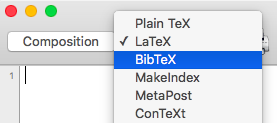
\includegraphics[height=2.2cm]{bibtex-texshop}
  \qquad
  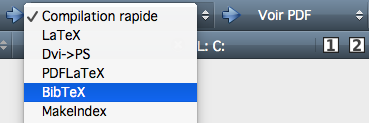
\includegraphics[height=2.2cm]{bibtex-texmaker}
  \caption{Interfaces de sélection du programme {\BibTeX} dans TeXShop
    (à gauche)
    et Texmaker (à droite)}
  \label{fig:bibliographie:editeurs}
\end{figure}

On trouvera des informations additionnelles, notamment sur des sources
de données bibliographiques et des outils de gestion des bases de
données, dans la section %
\doc[Gestion de la bibliographie]{}{https://fr.wikibooks.org/wiki/LaTeX/Gestion_de_la_bibliographie} %
de \citeauthor{wikilivres:latex}.



%%%
%%% Exercices
%%%

\section{Exercices}
\label{sec:bibliographie:exercices}

\Opensolutionfile{solutions}[solutions-bibliographie]

\begin{Filesave}{solutions}
\section*{Chapitre \ref*{chap:bibliographie}}
\addcontentsline{toc}{section}{Chapitre \protect\ref*{chap:bibliographie}}

\end{Filesave}

\begin{exercice}
  Composer des entrées de base de données pour les références
  bibliographiques suivantes.
  \begin{enumerate}
  \item \nolink{\bibentry{Mittelbach:floats:2014:nourl}}

    \emph{Astuce}: cette entrée est un article tiré d'une revue
    scientifique.

  \item \nolink{\bibentry{memoir}}

    \emph{Astuces}: traiter cette entrée comme un livre et utiliser le
    champ \code{note} pour consigner la remarque qui se trouve à la
    fin de la notice.

  \item \nolink{\bibentry{pstricks}}

    \emph{Astuces}: utiliser le type de document \code{Manual};
    attention à la casse de certains mots; on obtient le symbole {\ss}
    avec la commande \cmdprint{\ss}.
  \end{enumerate}
  \begin{sol}
    On trouve les champs obligatoires et optionnels pour chaque type
    d'entrée dans %
    \doc[Wikipedia]{}{https://fr.wikipedia.org/wiki/BibTeX}. %
    La clé est laissée vacante dans les réponses ci-dessous.
    \begin{enumerate}
    \item On utilise le type \code{Article} pour cette entrée.
\begin{lstlisting}[language=]
@Article{,
  author =  {Frank Mittelbach},
  title =   {How to Influence the Position of Float
             Environments Like Figure and Table In
             {\LaTeX}?},
  journal = {{TUG}boat},
  year =    2014,
  volume =  35,
  number =  3,
  pages =   {258-254},
  language = {english}}
\end{lstlisting}

    \item On utilise le type \code{Book} pour cette entrée.
\begin{lstlisting}[language=]
@Book{,
  author =  {Peter Wilson},
  title =   {The Memoir Class for Configurable
             Typesetting},
  publisher = {The Herries Press},
  year =     2013,
  edition =  8,
  note =    {Maintained by Lars Madsen},
  url =     {http://www.ctan.org/pkg/memoir/},
  language = {english}}
\end{lstlisting}

    \item La réponse ci-dessous contient les prénoms des auteurs,
      simplement afin d'illustrer que {\BibTeX} sait les abréger au
      moment de composer la notice bibliographique. Remarquer
      l'utilisation des accolades \verb={ }= dans le titre pour
      préserver la casse de «PSTricks» et de «PostScript».
\begin{lstlisting}[language=]
@Manual{,
  author = {Timothy {V}an Zandt and Denis Girou and
            Herbert Vo{\ss}},
  title =  {{PSTricks} --- {PostScript} Macros for
            Generic {\TeX}},
  year =   2014,
  url =    {http://www.ctan.org/pkg/pstricks-base/},
  language = {english}}
\end{lstlisting}
    \end{enumerate}
  \end{sol}
\end{exercice}

\begin{exercice}[nosol]
  Utiliser pour cet exercice le fichier
  \fichier{exercice\_gabarit.tex} ainsi que la base de données
  bibliographique crée à l'exercice précédent.
  \begin{enumerate}
  \item Créer un document simple comprenant des références à une ou
    plusieurs des entrées bibliographiques de l'exercice précédent.
    Compiler le document en suivant les étapes mentionnées à la
    \autoref{sec:bibliographie:bibtex} en utilisant tour à tour les
    styles par défaut \code{plain}, \code{unsrt}, \code{alpha} et
    \code{abbrv}.
  \item Charger dans le document le paquetage \pkg{natbib} (avant
    \pkg{babel}) et utiliser le style de bibliographie \code{francais}
    fourni par \pkg{francais-bst} (installé par défaut dans
    {\TeX}~Live). Recompiler le document et observer les différences
    par rapport aux documents produit en a).
  \end{enumerate}
\end{exercice}

\begin{exercice}[nosol]
  À partir d'un gabarit fourni avec la classe \class{ulthese},
  produire un document simple contenant une bibliographie.
\end{exercice}

\Closesolutionfile{solutions}

%%% Local Variables:
%%% mode: latex
%%% TeX-master: "formation-latex-ul"
%%% TeX-engine: xetex
%%% coding: utf-8
%%% End:
